% Range--inertial acquisition and closed-loop recovery: distinct manuscript revision.
% Compile twice with pdfLaTeX. The two vector figures live in recovery_window_revision_figures/.
\documentclass[conference,letterpaper,10pt]{IEEEtran}
\usepackage{amsmath,amssymb,bm,booktabs,array,graphicx,cite}
\usepackage{balance}
\usepackage[hidelinks]{hyperref}
% Use the standard TeX Live monospace face for short source revisions.
\renewcommand{\ttdefault}{cmtt}
\hypersetup{pdftitle={Range--Inertial Position Acquisition with Profiled Yaw and a Rotating Bias Model},pdfauthor={Anonymous Authors}}
\newcommand{\R}{\mathbb R}
\newcommand{\rz}{R_z}
\newcommand{\norm}[1]{\left\lVert#1\right\rVert}
\newcommand{\sk}[1]{[#1]_\times}
\newtheorem{proposition}{Proposition}
\title{Range--Inertial Position Acquisition\\with Profiled Yaw and a Rotating Bias Model}
\author{\IEEEauthorblockN{Anonymous Authors}}
\begin{document}
\maketitle
\raggedbottom
\begin{abstract}
A single ultra-wideband tag can recover horizontal position without resolving heading accurately enough to reset a navigation filter. A squared-range relaxation eliminates polynomial translation and supplies one yaw candidate; a robust fit to the original distances then allows a constant accelerometer bias to rotate with the body. With the same yaw candidate, horizontal endpoint RMSE falls from 1.625 to 0.159\,m on six Delft flights and from 2.930 to 1.631\,m against a prism reference on ten outdoor recordings. An unrestricted quadratic correction matches horizontal accuracy on Delft, so the evidence supports correcting the inertial shape more strongly than it identifies a unique bias model. In shared range windows, two published quadrotor estimators still achieve lower horizontal RMSE. Replacing the interval posterior of a single invariant filter helps all six Delft flights after a 20\,s outage but can severely degrade later tracking outdoors. We therefore recommend the window model for position acquisition, without treating its endpoint improvement as evidence for routine filter or heading resets.
\end{abstract}
\begin{IEEEkeywords}
Ultra-wideband, inertial navigation, initialization, moving-horizon estimation, invariant Kalman filtering.
\end{IEEEkeywords}

\section{Introduction}
When two-way ranges (TWR) return after an interruption, the first few anchors may locate a tag horizontally while leaving its heading ambiguous. Two decisions follow: how to extract a position from the arriving window, and whether to change the state already being propagated by an inertial filter. A good answer to the first question need not be a good answer to the second. A window estimate arrives late; it may also contain the same information as the current posterior.

We study a single tag, known anchor positions and asynchronous ranges. The window uses a gravity-aligned inertial frame but need not have a known yaw or translational velocity. We retain the profiled yaw seed of the affine initializer. Our principal change is the trajectory fitted to the original ranges: it may deviate from its nominal inertial shape through a body-fixed acceleration offset. A quadratic world-frame correction provides a strong alternative. A site-specific radio mean is optional; its contribution is measured separately from motion correction.

Our contributions are (i) a derivation connecting yaw profiling, bias sensitivity and loss of heading information; (ii) matched physical endpoint tests separating the benefit of the motion model from the cost and reliability of the yaw seed; and (iii) comparisons with published estimators and a test of posterior replacement in one InEKF. Horizontal position is the primary outcome; vertical error is reported separately. We make no physical heading claim on data without an independent attitude reference.

\section{Related methods and comparison targets}
Pacholska, D\"umbgen and Scholefield recover trajectory-basis coefficients from distances alone by lifting their quadratic terms~\cite{pacholska}. This provides a window baseline that does not require an IMU. Our relaxation instead uses the measured inertial shape and leaves a unit-circle variable for yaw. Other range initializers use multiple tags or constrained body motion~\cite{goudar}. Ranging--inertial factor graphs can initialize and subsequently smooth an entire trajectory~\cite{jiang}; their joint optimization motivates testing whether the endpoint is suitable for filter handoff.

Pfeiffer \emph{et al.} published a moving-horizon estimator (MHE), a companion EKF and the Delft quadrotor data~\cite{pfeiffer,delftdata}. Their estimator uses vehicle dynamics and a short rolling horizon. We compare their estimators at the same endpoint times and distinguish their published replay inputs from TWR and IMU alone. Oursland and Mehrabian's InEKF~\cite{oursland} is an online reference for lever-arm time differences of arrival (TDoA), not an absolute-range window solver. The quadratic observer of Theodosis \emph{et al.}~\cite{theodosis} estimates position and velocity from known acceleration and one range. The project's multi-anchor lifted capture is not an author implementation from either paper.

\section{Window model and candidate generation}
Let $a_i$ be the anchor and $z_i$ the range at transaction time $t_i$. The nominal inertial dynamics and observation are
\begin{gather}
 \dot R=R\sk{\omega_m-b_g},\quad \dot v=R(f_m-b_a)+g,\quad \dot p=v,\label{eq:ins}\\
 z_i=D_i+\mu_{a_i}(D_i,n_i)+e_i,\quad D_i=\norm{p_i-a_i}.\label{eq:obs}
\end{gather}
Here $n_i=(p_i-a_i)/D_i$ and $g=-9.81e_3$\,m/s$^2$. The TWR window sets the tag lever arm to zero. Write $R(t)=\rz(\psi)Q(t)$ to separate the unknown yaw from nominal tilt and gyro integration. At the last available instant $T$, let $\tau_i=t_i-T\le0$. Reanchoring the nominal double integral to remove endpoint position and velocity gives $d(T)=\dot d(T)=0$. With correct tilt, biases and consistent sample convention the affine trajectory is
\begin{equation}
 p_i=p_T+\tau_i v_T+\rz(\psi)d_i.                    \label{eq:affine}
\end{equation}

\subsection{A cheap yaw seed}
For candidate generation write $p_i=c(t_i)+\rz(\psi)d_i$ with $c(t)=\sum_{j=0}^K c_j\tau^j$. Use constant anchor corrections $r_i=z_i-\beta_i$ at this stage and form
\begin{equation}
 y_i=\tfrac12(r_i^2-\sigma_i^2-\norm{a_i}^2-\norm{d_i}^2)+a_{iz}d_{iz}.
\end{equation}
In the noiseless case ($\sigma_i=0$ in the identity), expansion gives $y=B\nu+Dc+Cu$. Here $u=(\cos\psi,\sin\psi)^\top$ and the row blocks are
\begin{align}
 B_i&=[\{\tau_i^\ell\}_{\ell=0}^{2K},\{\tau_i^j d_{ix},\tau_i^j d_{iy}\}_{j=0}^{K}],\nonumber\\
 D_{ij}&=\tau_i^j[-a_{ix},-a_{iy},d_{iz}-a_{iz}],\nonumber\\
 C_i&=[-a_{ix}d_{ix}-a_{iy}d_{iy},\,a_{ix}d_{iy}-a_{iy}d_{ix}].
\end{align}
The auxiliary coefficients $\nu$ contain the polynomial terms in $\frac12\norm{c(t)}^2$ and horizontal cross terms. They are independent variables only in the relaxation. With diagonal whitener $W$, let $L=W[B\ D]$, $P=I-LL^\dagger$, $\bar C=PWC$ and $\bar y=PWy$. The seed solves
\begin{equation}
  \min_{\|u\|=1}\|\bar y-\bar C u\|^2 .               \label{eq:circle}
\end{equation}
For $H=\bar C^\top\bar C$, $h=\bar C^\top\bar y$, $\Delta=H_{22}-H_{11}$ and $q=\tan(\psi/2)$ the stationary polynomial is
\begin{align}
 0={}&(H_{12}+h_2)q^4+2(h_1-\Delta)q^3-6H_{12}q^2 \nonumber\\
    &+2(h_1+\Delta)q+(H_{12}-h_2).
\end{align}
Evaluating the real roots and the omitted angle $\pi$ solves the relaxed circle problem globally. The variance of the centered half-squared Gaussian inlier error is $D_i^2\sigma_i^2+\sigma_i^4/2$; the whitening weight uses $\max(r_i,\sigma_i)$ for the unknown $D_i$. We project by SVD, retaining singular values above $10^{-10}s_{\max}$. Profile-1 passes a single candidate and a common robust constant-velocity (CV) translation seed to the nonlinear fit; the latter has no global certificate.

\begin{proposition}
For exact noiseless data satisfying the polynomial model, $\operatorname{rank}(\bar C)=2$ suffices for exact recovery of $u$. With yaw fixed, translation is unique if $(I-WB(WB)^\dagger)WD$ has rank $3(K+1)$.
\end{proposition}
\begin{IEEEproof}
The physical solution gives zero projected residual. Any minimizer satisfies $\bar C(u-u_\star)=0$. Full column rank forces equality. Eliminating $\nu$ from the remaining equations gives the translation condition.
\end{IEEEproof}
These conditions apply to the exact candidate model, not to an erroneous measured inertial shape.

\subsection{Fit the physical trajectory to the original ranges}
A constant accelerometer error in the body frame need not be a constant world acceleration. For a constant perturbation $\delta b_a$ over the window,
\begin{align}
 B_i^a&=\int_{t_i}^{T}(s-t_i)Q(s)\,ds,\label{eq:biasint}\\
 p_i&=p_T+\tau_i v_T+\rz(\psi)[d_i-B_i^a\delta b_a]. \label{eq:bias}
\end{align}
This is the endpoint-reanchored double integral of the accelerometer error under the nominal rotation. It is exact for that error with correct gyro, tilt and consistent discretization; it does not model gyro drift or identify the fitted $\delta b_a$ as the true sensor bias. Where independent calibration logs are available we use
\begin{equation}
 \mu_a(D,n)=\beta_a+s_a(D-\bar D_a)+\kappa_a^\top n. \label{eq:mean}
\end{equation}
The slope and directional term are empirical, not surveyed anchor corrections. For an uncalibrated site we set $\mu_a=0$. The raw-range refinement solves
\begin{align}
 \min_{p_T,v_T,\psi,\delta b_a}\;&\sum_i\rho_2\!\left(
      \frac{D_i+\mu_{a_i}(D_i,n_i)-z_i}{\sigma_{a_i}}\right)
       +\frac{\|\delta b_a\|^2}{2\sigma_b^2},\nonumber\\[-2pt]
 &\hspace{18mm}\sigma_b=0.10\,\mathrm{m/s^2}.             \label{eq:raw}
\end{align}
Only the radio terms use Huber loss with normalized threshold 2. The Gaussian working prior is held fixed between Delft and QDrone. The optimizer differentiates both distance and direction in~\eqref{eq:mean}. The $K=2$ control adds $\tfrac12\tau_i^2c_W$ to~\eqref{eq:affine} with no prior on the three world-frame coefficients. Both use the same translation seed and cap of 120 evaluations per start. Equations~\eqref{eq:biasint}--\eqref{eq:raw}, rather than a new yaw search, distinguish this fit from the affine baseline.

\subsection{What does a good position say about heading?}
Let $[J_n\ j_\psi]$ be the locally reweighted raw-range Jacobian. Include free position, velocity and bias columns in $J_n$. The data-only conditional heading curvature is
\begin{equation}
 \mathcal I_{\psi\mid n}=\|(I-J_nJ_n^\dagger)j_\psi\|^2 . \label{eq:info}
\end{equation}
Adding a bias prior can increase curvature without adding heading information from the data. Even large local curvature cannot exclude a distant yaw mode.
\begin{proposition}
Under constant attitude and measured specific force, unrestricted constant accelerometer bias makes yaw unidentifiable from zero-lever-arm position ranges even with noiseless dense data and nondegenerate anchors.
\end{proposition}
\begin{IEEEproof}
For any alternative yaw $\psi'$ choose
\begin{equation*}
b'_a=f_m-Q^\top\rz(\psi')^\top\rz(\psi)Q(f_m-b_a).
\end{equation*}
It is constant and preserves world acceleration. With the same starting position and velocity it preserves every range.
\end{IEEEproof}
More generally, adding a degree-$K$ polynomial $b(t)$ to $d$ has no effect on the translation-profiled raw objective: replace $c(t)$ by $c(t)-\rz(\psi)b(t)$. The change to $j_\psi$ lies in the nuisance span and disappears from~\eqref{eq:info}. The relaxed circle cost has the same invariance at fixed range weights: changes to the cross terms in $B$ are polynomials of degree at most $2K$, changes to $D$ lie in that same span, and changes to $y,C$ are eliminated by $P$. This invariance assumes free polynomial coefficients, not the prior-constrained bias fit. When $\|\dot Q\|_2\le\Omega$,
\begin{equation}
 \|B_i^a-\tfrac12(T-t_i)^2Q(T)\|_2\le\tfrac{\Omega}{6}(T-t_i)^3 . \label{eq:bound}
\end{equation}
This follows by integrating $\|Q(s)-Q(T)\|_2\le\Omega(T-s)$. A free quadratic can therefore approximate the leading bias-induced shape change without identifying a body bias.
\section{Matched position-acquisition experiments}
\subsection{Inputs, clocks and experimental units}
Delft~\cite{delftdata} provides two recordings for each of six motions. Earlier recordings supply radio calibration; the later recording of each motion is evaluated. We use the same fixed 0.20\,s clock alignment, truth-supported valid interval, approximately 1.5\,s static prefix and held IMU samples for both window models. Evaluation truth scores the outputs; it does not fit a test trajectory. These six same-date flights were seen in prior development. Each supplies 11 windows: 2 and 4\,s ending at 5\,s, and 2, 4 and 8\,s ending at 10, 20 and 30\,s on the retained clock. We use the last available sample at each endpoint. Two layouts (eight anchors or the four lowest) give 132 layout-specific windows from 66 physical windows. Four equivalent inertial yaw coordinates exercise the optimizer on the same data; the resulting 528 configurations are not independent acquisitions.

QDrone supplies ten outdoor recordings at a field, a building, a bridge and a tunnel~\cite{qdrone}. Each contributes 2, 4 and 8\,s windows ending at the sensor-coverage midpoint: 30 windows but only ten distinct endpoint instants. The registered total-station prism is a proxy. The exact prism--IMU--antenna transform, raw total-station timestamps and attitude truth are unavailable. No truth alignment or Delft calibration is transferred. All fits use the same initialization prefix, zero radio mean and a $0.30$\,m radio scale. This panel tests transfer of the motion correction, not of the directional radio calibration.

Horizontal error is $e_{xy}=\|\hat p_{T,xy}-p^*_{T,xy}\|$. Endpoint tables report $\sqrt{\operatorname{mean}(e_{xy}^2)}$, and analogously for Z and 3D. For trackers we instead score a time interval within each flight and specify the across-flight aggregation. Methods see no measurements after the evaluation timestamp. We do not use overlapping windows as independent population replicates.

\begin{table*}[t]
\caption{Paired physical endpoint RMSE (m). Both fits use a single Profile-1 yaw candidate and the same CV translation policy. Delft averages equivalent yaw coordinates; QDrone uses its recorded frame and a prism proxy. The QDrone vertical result is retained.}
\label{tab:end}\centering
\begin{tabular}{lrrrrrrr}
\toprule
&\multicolumn{3}{c}{Affine window}&\multicolumn{3}{c}{Body-bias window}&\\
\cmidrule(lr){2-4}\cmidrule(lr){5-7}
Data / geometry&XY&Z&3D&XY&Z&3D&Configurations\\
\midrule
Delft, eight anchors&1.585&0.758&1.757&0.116&0.209&0.239&264\\
Delft, four lowest anchors&1.664&1.163&2.030&0.192&0.526&0.560&264\\
Delft, both layouts&1.625&0.981&1.898&0.159&0.400&0.431&528\\
QDrone, four sites&2.930&1.655&3.365&1.631&1.779&2.414&30\\
\bottomrule
\end{tabular}
\end{table*}

\subsection{Physical endpoints: sources of the gain}
On Delft the paired horizontal RMSE decreases by 90.2\% (Table~\ref{tab:end}); 440 of 528 coordinate/layout/window pairs improve. All six flights improve in aggregate for XY, Z and 3D. Long windows account for much of the gain: at 2, 4 and 8\,s XY changes by $0.222\to0.164$, $0.709\to0.175$ and $2.991\to0.126$\,m. All 144 eight-second configurations improve horizontally. The totals of 32,632 and 32,789 function evaluations both include two common CV solves. Their difference of 0.48\% is not a timing comparison: the bias sensitivity and directional mean cost extra per evaluation.

\begin{figure*}[t]
\centering
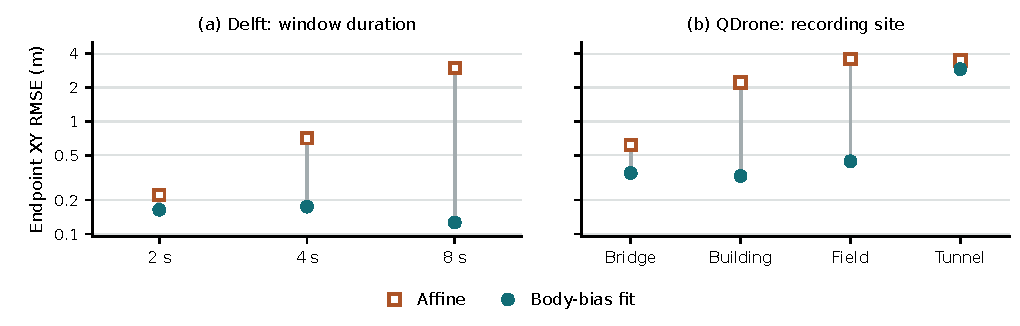
\includegraphics[width=.92\textwidth]{recovery_window_revision_figures/paired_xy.pdf}
\caption{Same single yaw candidate before and after changing the fitted trajectory. Delft uses separate calibration flights and both anchor layouts. QDrone uses a neutral radio mean for both fits; each site pools three windows per recording midpoint. The shared vertical scale is logarithmic.}
\label{fig:paired}
\end{figure*}

QDrone pooled proxy XY improves by 44.3\%. Eight-second XY falls from 4.312 to 1.605\,m; at two seconds it rises from 1.634 to 1.659\,m. All four site aggregates improve (Fig.~\ref{fig:paired}), but the tunnel remains near 3\,m and vertical RMSE increases. With four yaw starts on both sides, all ten recordings improve in aggregate across their three lengths, but only 20 of 30 individual windows improve. The data do not support a universal short-window advantage.

\begin{table}[t]
\caption{Delft controls at a fixed yaw coordinate: 66 windows per layout, four starts per fit. XY and 3D are RMSE in metres.}
\label{tab:model}\centering\small
\begin{tabular}{lrrrr}
\toprule
&\multicolumn{2}{c}{Eight anchors}&\multicolumn{2}{c}{Four lowest}\\
\cmidrule(lr){2-3}\cmidrule(lr){4-5}
Model / radio mean&XY&3D&XY&3D\\\midrule
Affine / constant&1.631&1.799&1.665&2.029\\
Free quadratic / constant&.127&.320&.201&.924\\
Body bias / constant&.133&.279&.203&.874\\
Free quadratic / directional&.111&.273&.188&.591\\
Body bias / directional&.116&.239&.192&.560\\
\bottomrule\end{tabular}
\end{table}
Table~\ref{tab:model} separates the two changes. With the radio mean held constant, either motion correction removes most of the XY error. Under the same directional mean the free quadratic has slightly lower pooled XY than body bias (0.155 versus 0.159\,m); body bias gives lower 3D (0.431 versus 0.460\,m). Each wins on XY in three flights. When calibration excludes the target motion, switching from a constant to a directional mean still reduces body-bias XY from $0.135$ to $0.119$\,m (eight anchors) and $0.204$ to $0.199$\,m (four). This is cross-motion validation within one room.

\subsection{Seed reliability with the objective held fixed}
\begin{table}[t]
\caption{Delft seed policies for the same body-bias objective: 528 configurations. Evaluations include CV solves; misses are relative to the best observed objective.}
\label{tab:seed}\centering\small\setlength{\tabcolsep}{4.5pt}
\begin{tabular}{lrrrr}
\toprule Seed&Misses&Evaluations&XY (m)&3D (m)\\\midrule
One local yaw&7&36,313&.154&.429\\
Profile-1&0&32,789&.159&.431\\
Four uniform yaws&0&86,508&.159&.431\\\bottomrule
\end{tabular}
\end{table}
A miss means $J-J_{\rm best}>10^{-4}(1+J_{\rm best})$ within the same objective. Profile-1 matches four uniform starts on the observed objective with 62.1\% fewer function evaluations (Table~\ref{tab:seed}). The local start has slightly lower aggregate physical error. The selected local, profiled and four-start solutions include 3, 4 and 0 nonconverged fits, respectively; all remain in the scores. On QDrone a subsequent seed-only check gives 1, 0 and 0 misses and 1,677, 1,429 and 4,174 evaluations. This is a check on the same recordings, not a new test set.

In a far-field affine simulation at 30\,m stand-off and a 3\,m anchor-height span, Profile-1 and two uniform starts both reach the best observed objective in all 200 trials; a single local start does so in 159. Median sequential desktop times on a separate timing subset are 47.1 and 66.6\,ms for Profile-1 and two starts. At a 0.1\,m height span Profile-1 still misses 12/200 times. These timing and capture figures apply to the affine simulation, not the real body-bias runs.
\section{Comparisons with published estimators}
\subsection{Same Delft endpoint: published TWR estimators}
Table~\ref{tab:published} compares the same 132 layout-specific time windows, without duplicating coordinate frames. Every method produces a finite estimate for every window. All rows in a given radio condition receive the same changed, positive range transactions, anchors, time convention and endpoint reference. Differences in the sensors and model priors are intrinsic to the methods and are stated below.

\begin{table*}[t]
\caption{Delft published-method comparison. Each triplet is endpoint XY, Z and 3D RMSE (m), 66 windows per layout. Constant = the same per-anchor offset estimated on earlier flights; raw = zero offset. No height input or online test-truth noise estimate. The two radio conditions form separate comparisons.}
\label{tab:published}\centering\small
\begin{tabular}{llrrrrrr}
\toprule
&&\multicolumn{3}{c}{Eight anchors}&\multicolumn{3}{c}{Four lowest anchors}\\
\cmidrule(lr){3-5}\cmidrule(lr){6-8}
Estimator / implementation&Radio mean&XY&Z&3D&XY&Z&3D\\\midrule
Pacholska et al., degree one, unweighted&Constant&.669&.425&.793&.689&5.803&5.844\\
Pacholska et al., degree one, author weights&Constant&.672&.411&.788&.676&6.268&6.305\\
Same solver, degree two (our setting)&Constant&.356&.491&.606&.474&7.982&7.996\\
Pfeiffer et al., author MHE&Constant&.121&.321&.343&.187&.876&.895\\
Pfeiffer et al., author EKF&Constant&.105&.231&.254&.188&.869&.889\\
Our single Profile-1 + body bias&Constant&.133&.245&.279&.204&.854&.878\\
\midrule
Pfeiffer et al., author MHE&Raw&.150&.549&.569&.219&.235&.321\\
Pfeiffer et al., author EKF&Raw&.172&.506&.534&.229&.243&.334\\
Our single Profile-1 + body bias&Raw&.205&.523&.562&.397&.241&.465\\
\bottomrule\end{tabular}
\end{table*}

\emph{Range-only reconstruction.} In the polynomial experiment of Pacholska \emph{et al.}~\cite{pacholska}, the two basis functions $(1,t)$ describe a line. Their published relaxation replaces the quadratic constraint $L=C^\top C$ for trajectory coefficients $C$ by independent coefficients. We evaluate the unweighted and author-weighted solves; the code's row weight is $1/\sqrt{r_i^2+0.1}$. Our numerically equivalent SVD implementation was compared with the literal author functions (commit \texttt{b2a2b58}) on 36 real fits; the largest relative coefficient discrepancy was $6.2\times10^{-12}$. As a stronger control we also prespecified $(1,t,t^2)$ in that same implementation. All 396 fits were full rank. This method uses no IMU, seed, height bound or subsequent raw-range fit. With the lowest four anchors many solutions have large vertical errors. We retain them: a full-rank least-squares system need not be well conditioned for physical height.

\emph{MHE and EKF with shared range inputs.} For Pfeiffer \emph{et al.}~\cite{pfeiffer} we call the original estimator classes, not a reimplementation (author commit \texttt{cb816bd}). The MHE retains its published 50\,Hz schedule, 20-node horizon, single gradient step and RANSAC; the EKF runs at 100\,Hz. Each estimator restarts with the authors' zero position/velocity and level, zero-yaw attitude; the external 2/4/8\,s data window does not change the MHE's internal 0.4\,s horizon. Both retain the authors' quadrotor thrust/drag model; the thrust proxy is formed from on-board acceleration, not supplied by an extra measured motor signal. We disable the auxiliary height input, use fixed or training-only radio scales and allow the final pending measurements to be consumed. Our solver uses its static-prefix tilt/bias estimate and gyro history, and estimates yaw freely. Measurement packets, radio offsets and endpoints are matched; attitude priors and computation are not identical. The MHE does not use radio standard deviations in its gradient. The last four-start reference and single-start results were not assumed equal: with raw lowest-four data their XY RMSE differs (0.303 versus 0.397\,m).

Both author estimators beat our single-window fit on horizontal RMSE for both layouts under both common radio conditions. With eight anchors and constant corrections the EKF, MHE and our fit have 65, 56 and 63 of 66 endpoints within 0.5\,m in 3D. All 264 single-start outputs are scored, including 64 final fits that hit the evaluation cap: 2/66 and 51/66 for raw eight and four anchors, and 0/66 and 11/66 for the constant-corrected layouts. The headline reduction in Table~\ref{tab:end} is relative to the affine initializer, not the best published tracker.

\emph{Native author replay, separate from the window test.} We also ran the authors' continuous \texttt{Drone} replay from its own start. It generates a height measurement from OptiTrack Z and computes a truth-dependent range variance used by the EKF. Each of the four endpoint times is counted once per flight, not once for each possible window length. On its native clock, eight-anchor XY/Z RMSE is $0.266/0.053$\,m for MHE and $0.253/0.054$\,m for EKF (24 endpoints each); retaining those estimates and rescoring on the common physical clock gives $0.237/0.052$ and $0.244/0.056$\,m. Prior history, height and timing differ from Table~\ref{tab:published}, so the native replay is reported separately. These numbers are our replay of released code, not the figures printed in the original paper.

\subsection{Oursland: author code and physical heading on Toronto}
We imported Oursland and Mehrabian's unchanged InEKF class~\cite{oursland} (commit \texttt{f3b664e}) on Toronto UTIL~\cite{util}. The author-mode replay uses its native event queue, a known tag lever arm and TDoA differences, not TWR. We compare the unmodified recursion with a project variant that reserves packets for an XY update. Each group contains four flights and two initial-yaw interventions ($0^\circ,180^\circ$), with the same sensor-only initial state, author covariance and a $[10,20)$\,s radio outage. We score wrapped yaw differences against interpolated motion-capture attitude; in each case we compute time RMSE, then take the median of the eight case RMSEs. This is physical heading, not the imposed initial perturbation.

\begin{table}[t]
\caption{Toronto TDoA: median post-recovery [26,45) s XY RMSE (m) and physical yaw RMSE (degrees). Each cohort contains eight paired cases.}
\label{tab:oursland}\centering\small
\begin{tabular}{lrrrr}
\toprule
&\multicolumn{2}{c}{Primary}&\multicolumn{2}{c}{Complementary}\\
\cmidrule(lr){2-3}\cmidrule(lr){4-5}
Method&XY&Yaw&XY&Yaw\\\midrule
Oursland, author code&.112&5.93&.0705&7.22\\
Same code + reserved XY&.087&6.80&.0709&6.22\\\bottomrule
\end{tabular}
\end{table}
Only three of eight primary cases improve in paired post-recovery XY, despite the lower aggregate median; the complementary XY result is essentially unchanged. This does not justify a routine heading reset. The conference paper separately reports 0.08 versus 1.34\,rad RMS at $180^\circ$ initialization for its InEKF versus its ESKF comparator~\cite{oursland}. Its run population and angular statistic differ from our wrapped-yaw panel. We do not infer a TWR ranking from the Toronto numbers.

A separate comparison on the four primary recordings paired the author recursion with project position/velocity and full-attitude handoff policies, using the same native event queue, initial covariance and nominal/$180^\circ$ interventions. Scoring starts at 2, 16 and 26\,s for weak startup, dynamic handoff and outage recovery, respectively. The author's median post-window yaw RMSEs were $6.72^\circ$, $6.66^\circ$ and $5.93^\circ$; full attitude handoff gave $32.97^\circ$, $47.24^\circ$ and $65.42^\circ$. In the outage group, a position/velocity handoff retaining the current attitude lowered median XY from 0.112 to 0.087\,m but raised yaw to $40.15^\circ$. These are comparisons between complete policies, not the isolated effect of changing a single yaw value.

\begin{table*}[t]
\caption{Single-filter recovery on real TWR. Each entry is median over flights of within-interval XY RMSE (m), scored at 20\,Hz on the last emitted state. First 2\,s: H and W are identical. Later columns show identical prehistory without replacement (H), with replacement (W), and the old lifted strong baseline (L). Windows are relative to the return of radio data.}
\label{tab:loop}\centering\small
\begin{tabular}{llrrrrrrrr}
\toprule
&&\multicolumn{2}{c}{0--2\,s}&\multicolumn{3}{c}{2--5\,s}&\multicolumn{3}{c}{6--11\,s}\\
\cmidrule(lr){3-4}\cmidrule(lr){5-7}\cmidrule(lr){8-10}
Site&Gap (s)&H/W&L&H&W&L&H&W&L\\\midrule
Delft&2&.106&.142&.090&.089&.102&.094&.093&.094\\
&5&.179&.196&.088&.087&.102&.093&.093&.093\\
&10&.362&.230&.116&.087&.101&.095&.092&.092\\
&20&15.832&3.015&16.451&.109&.103&39.429&.092&.092\\
\midrule
QDrone&2&.181&.626&.119&.622&.621&.551&.551&.551\\
&5&.279&.614&.117&.622&.617&.545&.545&.545\\
&10&.860&.869&.623&.623&.620&.635&.547&.544\\
&20&1.391&1.048&.620&.620&.619&.577&.533&.536\\
\bottomrule\end{tabular}
\end{table*}

\begin{figure*}[t]
\centering
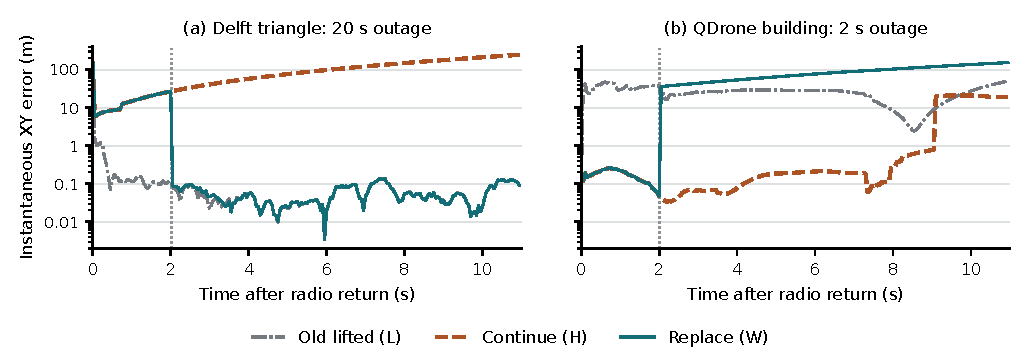
\includegraphics[width=.92\textwidth]{recovery_window_revision_figures/closed_loop_xy.pdf}
\caption{Online outputs after the same pre-outage history: W and H agree until the dotted handoff time, then recurse independently. Left: the first Delft flight in the protocol. Right: the QDrone case with the largest measured late paired deterioration after a 2\,s gap. The examples show both directions of change; they are not aggregate error estimates.}
\label{fig:closed}
\end{figure*}

\subsection{Theodosis: reconstruction of the published example}
Theodosis \emph{et al.}~\cite{theodosis} use a finite quadratic immersion for a linear system with quadratic output. Section VI of arXiv:2006.02688v2 uses known world acceleration, one absolute range and a continuous Riccati observer; it estimates $p,v$, not unknown 3D attitude. We reconstructed the equations, not author software. For the nine-state lifted system and scalar output we used $M_0=100 I_9$, $V=10^{-4}I_9$, $W=1$ in place of the incompatible six-dimensional printed matrices, and an all-zero initial estimate (unspecified in the example). At 20\,s the simulated position/velocity endpoint errors are 0.0957\,m and 0.0118\,m/s; the last-5\,s RMSEs are 0.1334\,m and 0.0223\,m/s. The 20\,s position does not meet a 1\,mm criterion. An extended simulation reaches $6.0\times10^{-6}$\,m at 100\,s. These numbers are local numerical results; the original reports convergence curves. They cannot be used as a real-flight heading benchmark.
\section{Can the window replace one InEKF posterior?}
\subsection{One estimator and one use of each measurement}
The online state is $(R,v,p,b_g,b_a)$ with 15-dimensional invariant error~\cite{barrau}. We retain one recursive posterior. A trigger occurs at startup or when the first range follows a gap longer than 1\,s. The native filter keeps predicting and emitting its own corrected states; an acquisition attempt waits for 2\,s of new sensor time, at least 16 ranges and four distinct anchors. For recovery, the checkpoint $c$ is the last complete posterior before the gap. Its measurements are already in the prior and are excluded from the replacement. Let $\mathcal E_{c:k}$ be the set of unique newly arrived range events after that checkpoint, including any events previously processed provisionally by the live estimator.

We recompute a local approximation to the \emph{conditional} interval posterior. Schematically, with the native discrete inertial transition $f_j$, process noise $w_j$ with covariance $S_w$, and local state difference $\boxminus$,
\begin{align}
 \min_{x_{c:k},w_{c:k-1}}\quad&
 \tfrac12\|x_c\boxminus\hat x_c\|^2_{P_c^{-1}}
 +\tfrac12\sum_{j=c}^{k-1}\|w_j\|^2_{S_w^{-1}}\nonumber\\
 &+\sum_{i\in\mathcal E_{c:k}}
 \rho_2\!\left(\frac{\|p_i-a_i\|+\beta_i-z_i}{\sigma_i}\right),
 \label{eq:replacement}\\[-3pt]
 &\hspace{4mm}x_{j+1}=f_j(x_j,u_j,w_j).\nonumber
\end{align}
The trigger uses observed outage length and anchor support; it does not establish that the native posterior actually needs replacement. We fix the rule, horizon, support and budget without selecting them using reference positions. Four iterated extended Kalman smoother passes use the same prior and factors. The linearized IMU transitions and process noise are those of the native filter, including bias random walks. The affine Profile-1 fit followed by the body-bias refinement supplies a reference trajectory; neither its estimate nor its bias prior is appended as an independent observation. The batch uses Huber weights, whereas native updates retain their innovation gate. The state, inertial model and raw range geometry are shared; the robust update policies differ.

At handoff we discard the live posterior for that interval, replace the state, both biases and the \emph{full} terminal covariance, transport the covariance into the invariant error coordinates, and continue normal recursion. The provisional outputs before handoff remain in the score. Repeated linearizations do not multiply a packet's information; the old posterior is not fused with the new one. We checked that four passes of a scalar unit-prior/unit-noise update still give variance $1/2$, and that navigation--bias cross blocks survive replacement. The covariance is a local approximation, not a calibrated confidence bound.

\subsection{A paired intervention on actual flights}
We remove all ranges for 2, 5, 10 or 20\,s ending at $t=25$\,s while retaining the IMU. Six Delft and ten QDrone recordings give 64 flight/gap cases. The test compares (H) the same profiled startup with native recursion at recovery, (W) that startup plus a profiled conditional replacement at recovery, and (L) the earlier project lifted capture followed by InEKF. This control matters: comparing a window-started tracker against a plain tracker that already failed at startup can credit recovery with an improvement it did not make. H and W have identical states, biases and covariance diagonals during the first two seconds in all 64 paired cases. A separate local-seed smoother on the same objective tests sensitivity to the numerical reference.

Table~\ref{tab:loop} requires at least 95\% reference coverage per interval. All six Delft flights qualify. At each QDrone gap, 7/10, 7/10 and 8/10 recordings qualify for the three intervals respectively; the others lack reference support. Four of the 40 QDrone recovery attempts lacked four observed anchors and kept the native filter. No numerical-failure case was dropped. There is no independent physical yaw truth for this TWR panel.

After a 20\,s Delft gap, the replacement improves all six late XY errors relative to H and recovers the lifted baseline's median late accuracy. It does not improve the first two seconds, and its worst 2--5\,s error is 3.48\,m versus 0.114\,m for L. On QDrone after a 2\,s gap, W has one late win, one tie and six losses against H; the worst paired deterioration is 102.85\,m. After a 5\,s gap the corresponding counts are again 1/1/6, with a 10.70\,m worst deterioration. Figure~\ref{fig:closed} shows how both an improvement and a failure persist beyond the handoff. Low excitation is consistent with weak curvature in~\eqref{eq:info}, but these diagnostics do not establish convergence to a local minimum: in one case the final pass still rotates the endpoint by $173^\circ$.

The earliest error also depends on the scoring clock. On the same Delft 20\,s lifted trajectories, the first-2\,s median is 3.015\,m with the frozen 20\,Hz hold, 0.979\,m on the original roughly 100\,Hz sample clock and 0.159\,m with the 20\,Hz grid offset by 25\,ms. The earliest hold can include the last outage prediction. For W the corresponding values are 15.832, 15.415 and 15.403\,m. The clocks change the magnitude but not this comparison. Finally, the 2\,s is a sensor-data wait, not end-to-end latency: median measured recovery-solver times were 1.58\,s on Delft and 6.34\,s on QDrone on this desktop under parallel load (maximum 24.44\,s on QDrone). New packets arriving during computation were not queued in the replay. No onboard real-time claim follows.

\section{Discussion and conclusion}
The large and repeatable change is in window-end position relative to a rigid affine inertial shape. It survives reduced anchor height diversity and a second measurement campaign, although short QDrone windows and its vertical coordinate do not improve. The free quadratic is competitive horizontally, and the published Pfeiffer estimators are stronger on horizontal accuracy under the two shared radio conditions. Profile-1 addresses a different issue: it reaches the best observed fitted objective reliably with fewer evaluations than uniform starts. It does not make heading observable.

The single-filter experiment establishes that a window can be incorporated coherently without duplicating measurements. It does not establish that doing so is beneficial as a default response to a gap. For immediate TWR recovery we therefore retain lifted capture as the benchmark; for native TDoA we retain the author's recursive InEKF. An accurate window position alone is not a reason to reset heading. A publishable deployment claim would require blind sites with measured IMU--tag extrinsics, independent clock and heading reference, and measured latency. Validation of the acquisition model and validation of a new recursive recovery policy should remain separate.
\balance
\begin{thebibliography}{10}
\bibitem{pacholska} M.~Pacholska, F.~D\"umbgen, and A.~Scholefield, \emph{Relax and Recover: Guaranteed Range-Only Continuous Localization}. IEEE Robot. Autom. Lett., vol.~5, pp.~2248--2255, 2020. \href{https://doi.org/10.1109/LRA.2020.2970952}{Article}; \href{https://github.com/LCAV/continuous-localization}{author code}.
\bibitem{goudar} A.~Goudar, F.~D\"umbgen, T.~D.~Barfoot, and A.~P.~Schoellig, \emph{Optimal Initialization Strategies for Range-Only Trajectory Estimation}. IEEE Robot. Autom. Lett., vol.~9, pp.~2160--2167, 2024, \href{https://doi.org/10.1109/LRA.2024.3354623}{doi:10.1109/LRA.2024.3354623}.
\bibitem{jiang} F.~Jiang, D.~Caruso, A.~Dhekne, Q.~Qu, J.~J.~Engel, and J.~Dong, \emph{Robust Indoor Localization with Ranging--IMU Fusion}. IEEE ICRA, 2024, pp.~11963--11969, \href{https://doi.org/10.1109/ICRA57147.2024.10611274}{doi:10.1109/ICRA57147.2024.10611274}.
\bibitem{pfeiffer} S.~Pfeiffer, C.~de~Wagter, and G.~C.~H.~E.~de~Croon, \emph{A Computationally Efficient Moving Horizon Estimator for Ultra-Wideband Localization on Small Quadrotors}. IEEE Robot. Autom. Lett., vol.~6, pp.~6725--6732, 2021. \href{https://doi.org/10.1109/LRA.2021.3095519}{Article}; \href{https://github.com/SUPfeiffer/uwb-simulator}{author code}.
\bibitem{delftdata} S.~Pfeiffer, C.~de~Wagter, and G.~C.~H.~E.~de~Croon, \emph{Data Underlying the Publication: A Computationally Efficient Moving Horizon Estimator for UWB Localization on Small Quadrotors}. 4TU.ResearchData, ver.~1, 2021, \href{https://doi.org/10.4121/14827680.v1}{doi:10.4121/14827680.v1}.
\bibitem{oursland} J.~Oursland and M.~Mehrabian, \emph{An Invariant Extended Kalman Filter for IMU--UWB Sensor Fusion}. IEEE RO-MAN, 2024, pp.~154--159. \href{https://doi.org/10.1109/RO-MAN60168.2024.10731434}{Article}; \href{https://github.com/oursland/imu-uwb-inekf}{author code}.
\bibitem{theodosis} D.~Theodosis, S.~Berkane, and D.~V.~Dimarogonas, \emph{State Estimation for a Class of Linear Systems with Quadratic Output}. IFAC-PapersOnLine, vol.~54, no.~9, pp.~261--266, 2021. \href{https://doi.org/10.1016/j.ifacol.2021.06.149}{Article}; \href{https://arxiv.org/abs/2006.02688v2}{version used}.
\bibitem{qdrone} Z.~Arjmandi \emph{et al.}, \emph{Benchmark Dataset of Ultra-Wideband Radio Based UAV Positioning}. IEEE ITSC, 2020. \href{https://doi.org/10.1109/ITSC45102.2020.9294440}{Article}; \href{https://benchmark.qdrone.ausmlab.com/datasets/}{dataset}.
\bibitem{util} W.~Zhao, A.~Goudar, X.~Qiao, and A.~P.~Schoellig, \emph{UTIL: An Ultra-Wideband Time-Difference-of-Arrival Indoor Localization Dataset}. Int. J. Robot. Res., 2024, \href{https://doi.org/10.1177/02783649241230640}{doi:10.1177/02783649241230640}.
\bibitem{barrau} A.~Barrau and S.~Bonnabel, \emph{The Invariant Extended Kalman Filter as a Stable Observer}. IEEE Trans. Autom. Control, vol.~62, pp.~1797--1812, 2017, \href{https://doi.org/10.1109/TAC.2016.2594085}{doi:10.1109/TAC.2016.2594085}.
\end{thebibliography}
\end{document}
